% !TeX root = proyecto.tex

%=========================================================
\chapter{Modelo dinámico}	
\label{cap:modDinamico}

\cdtInstrucciones{Presente la solución indicando el si esta se compone de varios sistemas, los subsistemas del sistema y si aplica, los módulos de los subsistemas.}

	Este capítulo describe en modelo dinámico del sistema. en el se detallan todos los escenarios de ejecución del sistema. La figura~\ref{fig:casosDeUso} muestra el diagrama general del sistema y sus subsistemas, y la figura~\ref{fig:casosDeUsoDetalle} muestra todos los casos de uso del sistema. En este documento solo detallamos los casos de uso del subsistema de gestión de cursos.
	
\begin{figure}[htbp]
	\begin{center}
		\fbox{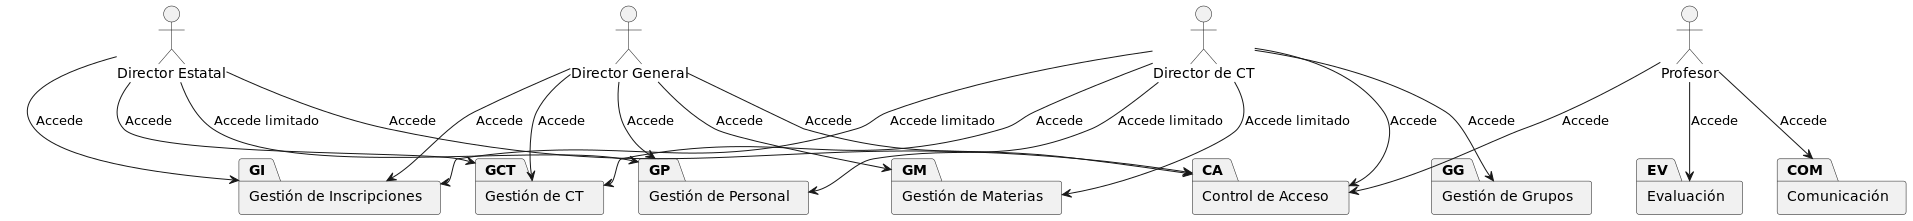
\includegraphics[width=.8\textwidth]{images/casosDeUso}}
		\caption{Diagrama de casos de uso del sistema.}
		\label{fig:casosDeUso}
	\end{center}
\end{figure}

\begin{figure}[htbp]
	\begin{center}
		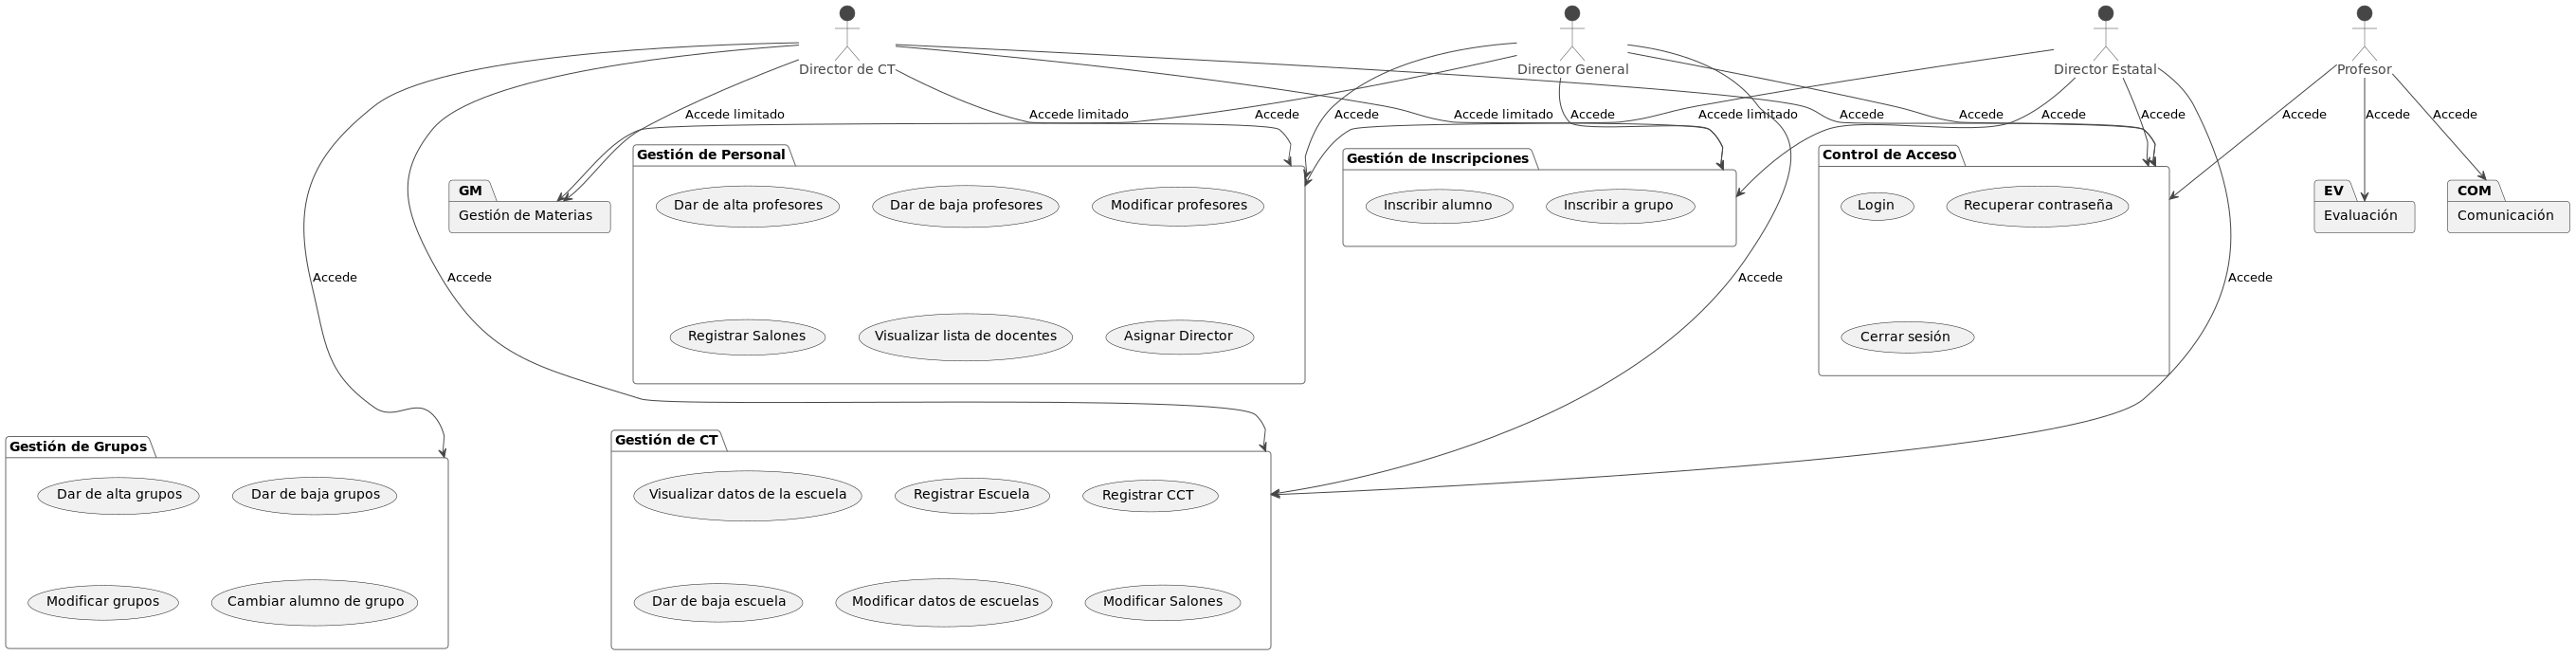
\includegraphics[angle=90, width=.7\textwidth]{images/casosDeUsoDetalle}
		\caption{Diagrama detallado del sistema.}
		\label{fig:casosDeUsoDetalle}
	\end{center}
\end{figure}

%---------------------------------------------------------
\section{Descripción de casos de uso}



A continuación se detallan los casos de uso.

%---------------------------------------------------------
% CASOS DE USO

%!TEX root = ../proyecto.tex

% Plantilla para caso de uso sencillo con ejemplos de comandos e intrucciones.
%-------------------------------------- COMIENZA descripción del caso de uso.

%\begin{UseCase}[archivo de imágen]{UCX}{Nombre del Caso de uso}{
%--------------------------------------
\begin{UseCase}{CUX}{Escriba el nombre del caso de uso}{
	% La descripción debe describir el evento de inicio del caso de uso, Breve descripción de la trayectoria y estado final del caso de uso.
}
	\UCitem{Versión}{\color{Gray}
		0.1	% Ponga un número de versión, 
	}\UCitem{Autor}{\color{Gray}
		Nombre del analista. % Analista responsable de especificar el CU
	}\UCitem{Supervisa}{\color{Gray}
		Nombre del analista revisor. % Analista responsable de verificar que está correcto.
	% TODO: Dar de alta al actor Usuario
	}\UCitem{Actor}{
		\hyperlink{IdDelActor}{Nombre del actor} % No olvide dar de alta el actor.
	}\UCitem{Propósito}{\begin{Titemize}%Indique los fines, objetivos, propósitos o valores agregados del Caso de uso.
		\Titem Propósito del caso de uso.
		\Titem ...
	\end{Titemize}
	}\UCitem{Entradas}{\begin{Titemize}
		% TODO: Dar de alta las entidades que se listan.
		\Titem \hyperlink{Entidad.Atributo}{Nombre del dato de entrada}. % El identificador no acepta acentos, espacios ni eñes.
		\Titem \hyperlink{Entidad.Atributo}{Nombre del dato de entrada}. % Liste todos los datos de entrada
		\end{Titemize}
	}\UCitem{Origen}{\begin{Titemize}
		\Titem Se introducen desde el teclado. % Indique por que medio se introducen los datos, 
		\Titem otros.          % Si es ḿas de uno indique que datos corresponden en cada medio de entrada.
	\end{Titemize}
	}\UCitem{Salidas}{\begin{Titemize}
		% TODO: Dar de alta las entidades que se listan.
		\Titem \hyperlink{Entidad.Atributo}{Nombre del dato de entrada}.
		\Titem Mensajes de error. % Indique por que medio se introducen los datos, 
		\Titem Datos que aparecen en pantalla.          % Si es ḿas de uno indique que datos corresponden en cada medio de entrada.
		\Titem Datos que aparecen en listas desplegables o tablas, etc.
		\Titem Datos que se imprimen o que se envía a otros sistemas.
	\end{Titemize}
	}\UCitem{Destino}{\begin{Titemize}
		\Titem Se muestra en la pantalla \IUref{IUX}{Nombre pantalla}.. % Indique por que medio se muestran los datos, 
		\Titem otros.          % Si es ḿas de uno indique que datos corresponden en cada medio de entrada.
	\end{Titemize}
	}\UCitem{Precondiciones}{\begin{Titemize}
		% Incluya Precondiciones lógicas, de negocio e incluso las que debe atender el usuario. 
		% Muchas precondiciones provienen de reglas de negocios, otras estarán asociadas a manejo de errores
		% Otras están relacionadas con casos de uso que deben ejecutarse previamente, como registrar un producto.
		\Titem Escriba la precondición.
	\end{Titemize}
	}\UCitem{Postcondiciones}{\begin{Titemize}
		% Indique todas las postcondiciones
		% por ejemplo, Cambios en el sistema
		% Cambios en la BD una vez terminado el CU
		% Efectos colaterales
		% Condiciones de término.
		\Titem Escriba todas las postcondiciones.
	\end{Titemize}
	}\UCitem{Errores}{\begin{Titemize}
		% Escriba todos los errores que puedan ocurrir en el sistema, para cada error recuerde:
		% Punerle un identificador
		% Describir la condición o escenario que detona el error
		% Describa la forma en que debe reaccionar el sitema: si la reaccion corresponde a varios pasos use mejor una trayectoria alternativa.
		% Relacione el error con la trayectoria principal.
		\Titem {\bf \hypertarget{CUX.E1}{E1}}: Condición que detona el error, reacción del sistema y regresa al paso \ref{UC1.etiqueta}.
		\Titem {\bf \hypertarget{CUX.E2}{E2}}: Condición que detona el error, reacción del sistema y termina el Caso de uso..
	\end{Titemize}
	}\UCitem{Tipo}{
		% Especifique el tipo de caso de us, puede ser: "Caso de uso primario" o 
		% "Viene de \\hyperref{CUY}{CUY nombre del CU}" cuando se desprende desde otro caso de uso mediante un extends.
		Caso de uso primario
	}\UCitem{Observaciones}{
		% Indique las observaciones al caso de uso, las cuales pueden ser:
		% - Ninguna
		% - Dudas sobre el procedimiento o la especificación.
		% - Issues detectados
		% - Suposiciones realizadas.
		% - Cualquier otra especificacion que considere pertinente que no pudo colocarse en los demás atributos del Caso de uso
		% - Aclaraciones.
		% - Notas para el usuario o desarrollador.
		% - Pendientes (TODO's) en caso de no usar los comentarios.
	}
\end{UseCase}

%--------------------------------------
\begin{UCtrayectoria}
	% Cada paso debe inicair con un Verbo en infinitivo, siempre especificando el objetivo del paso mas la accion en concreto.
	% \UCpaso[\UCactor] se refiere al actor y \UCpaso se refiere al sistema.
	% A continuación viene ejemplos de pasos:
	% En el siguiente paso: "Ingresa al sistema" es el objetivo del paso y "escribiendo la URL de la aplicación" es la acción en concreto.
	\UCpaso[\UCactor o \UCsist] VERBO EN INFINITIVO + (Acción del usuario) + (Acción dentro del sistema)
	\UCpaso[\UCactor] Ingresa al sistema escribiendo la URL de la aplicación.
	% En el siguinte paso se referencia una Interfaz:
	\UCpaso Solicita al usuario que se identifique mediante la pantalla \IUref{IU1}{Inicio de sesión}
	% En el siguiente paso está etiquetado para ser referenciado por un error o trayectoria alternativa:
	\UCpaso[\UCactor] \label{UCX.introduceDatos} Se identifica introduciendo su nombre de usuario y contraseña.
	% En el siguiente paso se usa el comando \IUbutton 
	\UCpaso[\UCactor] Solicita el ingreso al sistema presiona el botón \IUbutton{Ingresar}.
	% En el siguiente paso se referencía un error.
	\UCpaso Busca los datos del usuario identificado por el nombre de usuario introducido \ErrorRef{CUX}{E1}{No hay usuario}
	% En el siguiente paso se señala una trayectoria alternativa
	\UCpaso Verifica que el usuario especificado no esté inactivo \ErrorRef{CUX}{E2}{Usuario inactivo} \Trayref{CUX}{A}.
	% En el siguiente paso se referencían dos errores y una trayectoria alternativa.
	\UCpaso Verifica que la contraseña ingresada coincida con la almacenada \ErrorRef{CUX}{E3}{La contraseña no coincide}\Trayref{CUX}{B}.
	% En el siguiente paso se señala la incusión de otro CU
	\UCpaso[] Se ejecutan los pasos del caso de uso \UCref{CUY}{Nombre del caso de uso}.
	% En el siguiente paso se señala un mensaje.
	\UCpaso Muestra la pantalla \IUref{IU2}{Principal} con el mensaje \MSGref{MSG-001}{Bienvenida al usuario}.
\end{UCtrayectoria}


%--------------------------------------
% Las trayectorias alternativas se identifican con Letras: A, B, C, etc.
\begin{UCtrayectoriaA}{CUX}{LETRA}{Condición que hace que se ejecute esta trayectoria}
	\UCpaso Especifique los pasos  de la trayectoria.
	% Se puede desprender otra trayectria alternativa si es necesario.
	% Finalice la trayectoria indicando si la ejecución se integra a la trayectoria anterior o si termina la ejecución del CU.
	% Verifique que la redacción de la trayectoria deje en claro si el objetivo del CU se alcanzó o no.
	\UCpaso[] El Caso de Uso continúa en el paso \ref{UCX.introduceDatos}.
\end{UCtrayectoriaA}


%--------------------------------------
% Puntos de extensión

% Comente la siguiente sección en caso de que no hayan puntos de extensión o relaciones de tipo extends.
\subsection{Puntos de extensión}
\UCExtenssionPoint{
	% Cuando se dá la extensión del Caso de uso:
	El usuario no recuerda cual es su contraseña o sospecha que su usuario está bloqueado.
}{
	% Durante la región (en que pasos se puede dar la extensión):
	Del paso \ref{CUX.etiqueta} al paso \ref{CUX.etiqueta}.
}{
	% Casos de uso a los que extiende:
	\UCref{CUZ}{Nombre del caso de uso}.
}
		
		
		
%-------------------------------------- TERMINA descripción del caso de uso.
%!TEX root = ../proyecto.tex

% Plantilla para caso de uso sencillo con ejemplos de comandos e intrucciones.
%-------------------------------------- COMIENZA descripción del caso de uso.

%\begin{UseCase}[archivo de imágen]{UCX}{Nombre del Caso de uso}{
%--------------------------------------
\begin{UseCase}{CUX}{Escriba el nombre del caso de uso}{
	% La descripción debe describir el evento de inicio del caso de uso, Breve descripción de la trayectoria y estado final del caso de uso.
}
	\UCitem{Versión}{\color{Gray}0.1}% Ponga un número de versión, 
	\UCitem{Estatus}{\color{Gray}.}
	\UCitem{Prioridad}{\color{Gray}.}
	\UCitem{Usuario}{\color{Gray}Nombre del usuario o usuarios} % Usuarios que dieron la información para el CU.
	\UCitem{Elaboró}{\color{Gray}Nombre del analista} % Analista responsable de especificar el CU
	\UCitem{Supervisó}{\color{Gray}Nombre del analista revisor.} % Analista responsable de verificar que está correcto.
	\UCitem{Validó}{\color{Gray}Nombre del usuario o usuarios} % Usuarios que validan con su firma el caso de uso para su programación.
	\UCitem{Complejidad}{\color{Gray}.} % Muy alta, Alta, Media, Baja, Muy baja.
	\UCitem{Volatilidad}{\color{Gray}.} % Muy alta, Alta, Media, Baja, Muy baja.
	\UCitem{Madurez}{\color{Gray}.} % Muy alta, Alta, Media, Baja, Muy baja.
	\UCitem{Dificultades}{\color{Gray}
		\begin{Titemize}
			% Listar todas las dificultades que tiene el CU o moner la palabra ninguna.
			\Titem 
		\end{Titemize}
	}
	\UCitem{Proceso}{} % ID y nombre del proceso
	\UCitem{Sub-proceso}{} % ID y nombre del subproceso
	\UCitem{Área}{} % Nombre del área a la que oertenece el actor.
	% TODO: Dar de alta al actor Usuario
	\UCitem{Actor}{\hyperlink{IdDelActor}{Nombre del actor}} % No olvide dar de alta el actor.
	\UCitem{Tipo de operación}{} % Consulta, alta, baja, cambio, reporte, operacion del negocio, etc.
	\UCitem{Frecuencia}{ % Con que frecuencia o periodicidad minimá, promedio y máxima se ejecutará este caso de uso en el sistema
		\begin{Titemize}
			\Titem Mínimo:
			\Titem Promedio:
			\Titem Máximo:
		\end{Titemize}
	}
	\UCitem{Volumen}{ % Volumen mínimo, promedio y máximo de usuarios simultaneos o información se podría tener en la presente operación.
		\begin{Titemize}
			\Titem Mínimo:
			\Titem Promedio:
			\Titem Máximo:
		\end{Titemize}
	}
	\UCitem{Req. de usuario}{} % id y nombre de los requerimientos que satisface el CU.
	\UCitem{Fuentes}{
		\begin{Titemize}
			% Lista de fuentes documetnales que respaldan o en los que se basa el Caso de uso.
			\Titem 
		\end{Titemize}
	}	
	\UCitem{Propósito}{
		%Indique el fin, objetivo, propósito o valor agregado del Caso de uso.
		\begin{Titemize}
			\Titem 
		\end{Titemize}
	}
	\UCitem{Entradas}{
		\begin{Titemize}
			% TODO: Dar de alta las entidades que se listan.
			\Titem \hyperlink{Entidad.Atributo}{Nombre del dato de entrada}. % El identificador no acepta acentos, espacios ni eñes.
			\Titem \hyperlink{Entidad.Atributo}{Nombre del dato de entrada}. % Liste todos los datos de entrada
		\end{Titemize}
	}
	\UCitem{Origen}{\begin{Titemize}
			\Titem Se introducen desde el teclado. % Indique por que medio se introducen los datos, 
			\Titem otros.          % Si es ḿas de uno indique que datos corresponden en cada medio de entrada.
		\end{Titemize}} 
	\UCitem{Salidas}{\begin{Titemize}
			% TODO: Dar de alta las entidades que se listan.
			\Titem \hyperlink{Entidad.Atributo}{Nombre del dato de entrada}.
			\Titem Mensajes de error. % Indique por que medio se introducen los datos, 
			\Titem Datos que aparecen en pantalla.          % Si es ḿas de uno indique que datos corresponden en cada medio de entrada.
			\Titem Datos que aparecen en listas desplegables o tablas, etc.
			\Titem Datos que se imprimen o que se envía a otros sistemas.
	\end{Titemize}}
	\UCitem{Destino}{\begin{Titemize}
			\Titem Se muestra en la pantalla \IUref{IUX}{Nombre pantalla}.. % Indique por que medio se muestran los datos, 
			\Titem otros.          % Si es ḿas de uno indique que datos corresponden en cada medio de entrada.
	\end{Titemize}}
	\UCitem{Disparadores}{
	\begin{Titemize}
		% Liste y describa los escenarios en los que el actor debe ejecutar el caso de uso
		\Titem 
	\end{Titemize}
	}
	\UCitem{Precondiciones}{
		\begin{Titemize}
			% Incluya Precondiciones lógicas, de negocio e incluso las que debe atender el usuario. 
			% Muchas precondiciones provienen de reglas de negocios, otras estarán asociadas a manejo de errores
			% Otras están relacionadas con casos de uso que deben ejecutarse previamente, como registrar un producto.
			\Titem Escriba la precondición.
		\end{Titemize}
	}
	\UCitem{Condición de término}{
	\begin{Titemize}
		% Liste todos los efectos que un usuario (aunque sea otro actor) puede o debe ver en el sistema 
		% como consecuencia de la ejecución del cao de uso.
		\Titem 
	\end{Titemize}
	}
	\UCitem{Efectos colaterales}{
	\begin{Titemize}
		% 
		\Titem 
	\end{Titemize}
	}
	\UCitem{Postcondiciones}{
		\begin{Titemize}
			% Indique todas las postcondiciones que no haya listado en efectos colaterales o condiciones de término.
			% por ejemplo, Cambios en el sistema
			% Cambios en la BD una vez terminado el CU
			\Titem Escriba todas las postcondiciones.
		\end{Titemize}
	}
	\UCitem{Errores}{
		% Escriba todos los errores que puedan ocurrir en el sistema, para cada error recuerde:
		% Punerle un identificador
		% Describir la condición o escenario que detona el error
		% Describa la forma en que debe reaccionar el sitema: si la reaccion corresponde a varios pasos use mejor una trayectoria alternativa.
		% Relacione el error con la trayectoria principal.
		\begin{Titemize}
			\Titem {\bf \hypertarget{CUX.E1}{E1}}: Condición que detona el error, reacción del sistema y regresa al paso \ref{UC1.etiqueta}.
			\Titem {\bf \hypertarget{CUX.E2}{E2}}: Condición que detona el error, reacción del sistema y termina el Caso de uso..
		\end{Titemize}
	}
	\UCitem{Tipo}{
		% Especifique el tipo de caso de us, puede ser: "Caso de uso primario" o 
		% "Viene de \\hyperref{CUY}{CUY nombre del CU}" cuando se desprende desde otro caso de uso mediante un extends.
		Caso de uso primario
	}
	\UCitem{Casos de prueba}{
		% Liste todos los casos de prueba que identifica.
		\begin{Titemize}
			\Titem {\bf \hypertarget{CUX.E1}{E1}}: Condición que detona el error, reacción del sistema y regresa al paso \ref{UC1.etiqueta}.
			\Titem {\bf \hypertarget{CUX.E2}{E2}}: Condición que detona el error, reacción del sistema y termina el Caso de uso..
		\end{Titemize}
	}
	\UCitem{Consideraciones de diseño}{
	% Consideraciones tales como tiempo máximo de respuesta, retroalimentación, animaciones, cálculos complejos, operaciones asíncronas, etc.
	\begin{Titemize}
		\Titem ...
	\end{Titemize}
	}\UCitem{Impedimentos}{
	% Liste todos los impedimentos que conozca sobre este caso de uso
	\begin{Titemize}
		\Titem {\bf \hypertarget{CUX.E1}{E1}}: Condición que detona el error, reacción del sistema y regresa al paso \ref{UC1.etiqueta}.
		\Titem {\bf \hypertarget{CUX.E2}{E2}}: Condición que detona el error, reacción del sistema y termina el Caso de uso..
	\end{Titemize}
	}\UCitem{Preguntas}{
	% Liste todas las preguntas no contestadas del caso de uso
	\begin{Titemize}
		\Titem ...
	\end{Titemize}
	}\UCitem{Observaciones}{
		% Indique las observaciones al caso de uso, las cuales pueden ser:
		% - Ninguna
		% - Dudas sobre el procedimiento o la especificación.
		% - Issues detectados
		% - Suposiciones realizadas.
		% - Cualquier otra especificacion que considere pertinente que no pudo colocarse en los demás atributos del Caso de uso
		% - Aclaraciones.
		% - Notas para el usuario o desarrollador.
		% - Pendientes (TODO's) en caso de no usar los comentarios.
	}
\end{UseCase}

%--------------------------------------
\begin{UCtrayectoria}
	% Cada paso debe inicair con un Verbo en infinitivo, siempre especificando el objetivo del paso mas la accion en concreto.
	% \UCpaso[\UCactor] se refiere al actor y \UCpaso se refiere al sistema.
	% A continuación viene ejemplos de pasos:
	% En el siguiente paso: "Ingresa al sistema" es el objetivo del paso y "escribiendo la URL de la aplicación" es la acción en concreto.
	\UCpaso[\UCactor] Ingresa al sistema escribiendo la URL de la aplicación.
	% En el siguinte paso se referencia una Interfaz:
	\UCpaso Solicita al usuario que se identifique mediante la pantalla \IUref{IU1}{Inicio de sesión}
	% En el siguiente paso está etiquetado para ser referenciado por un error o trayectoria alternativa:
	\UCpaso[\UCactor] \label{UCX.introduceDatos} Se identifica introduciendo su nombre de usuario y contraseña.
	% En el siguiente paso se usa el comando \IUbutton 
	\UCpaso[\UCactor] Solicita el ingreso al sistema presiona el botón \IUbutton{Ingresar}.
	% En el siguiente paso se referencía un error.
	\UCpaso Busca los datos del usuario identificado por el nombre de usuario introducido 
	% En el siguiente paso se señala una trayectoria alternativa
	\UCpaso Verifica que el usuario especificado no esté inactivo  \Trayref{CUY}{A}.
	% En el siguiente paso se referencían dos errores y una trayectoria alternativa.
	\UCpaso Verifica que la contraseña ingresada coincida con la almacenada \Trayref{CUY}{B}.
	% En el siguiente paso se señala la incusión de otro CU
	\UCpaso[] Se ejecutan los pasos del caso de uso \UCref{CUY}{CUY Nombre del caso de uso}.
	% En el siguiente paso se señala un mensaje.
	\UCpaso Muestra la pantalla \IUref{IU2}{Principal} con el mensaje \hyperlink{MSG1}{MSG1 Bienvenida al usuario}.		
\end{UCtrayectoria}


%--------------------------------------
% Las trayectorias alternativas se identifican con Letras: A, B, C, etc.
\begin{UCtrayectoriaA}{CUY}{LETRA}{Condición que hace que se ejecute esta trayectoria}
	\UCpaso Especifique los pasos  de la trayectoria.
	% Se puede desprender otra trayectria alternativa si es necesario.
	% Finalice la trayectoria indicando si la ejecución se integra a la trayectoria anterior o si termina la ejecución del CU.
	% Verifique que la redacción de la trayectoria deje en claro si el objetivo del CU se alcanzó o no.
	\UCpaso[] El Caso de Uso continúa en el paso \ref{UCX.introduceDatos}.
\end{UCtrayectoriaA}


%--------------------------------------
% Puntos de extensión

% Comente la siguiente sección en caso de que no hayan puntos de extensión o relaciones de tipo extends.
\subsection{Puntos de extensión}
\UCExtenssionPoint{
	% Cuando se dá la extensión del Caso de uso:
	El usuario no recuerda cual es su contraseña o sospecha que su usuario está bloqueado.
}{
	% Durante la región (en que pasos se puede dar la extensión):
	Del paso \ref{CUX.etiqueta} al paso \ref{CUX.etiqueta}.
}{
	% Casos de uso a los que extiende:
	\UCref{CU3.4}{Consultar historial académico}.
}
		
		
		
%-------------------------------------- TERMINA descripción del caso de uso.
%\input{cu/cu-02}
%\input{cu/cu-03}
%\input{cu/cu-04}
%\input{cu/cu-05}
%\input{cu/cu-06}
%\input{cu/cu-07}
%\input{cu/cu-08}


